\section{Ground State Energy and Vacuum Amplitude}
\subsection{Meaning of the vacuum amplitude}
One of the first many-body problems to be tackled by the field theoretical diagram techniques was that of finding the ground state energy $E_0$ of a system of interacting fermions. The diagrammatic methods in this chapter provide a neat way of handling nuclear and electron interactions. In both cases, we can perform a partial sum over an infinite series of infinite terms and get a finite result. In order to do this, it is necessary to have a general way of writing down the nth-order term in the ordinary perturbation series for $E_0$,i.e., in
\begin{equation}E_{0}=W_{0}+\left\langle\Phi_{0}\left|H_{1}\right| \Phi_{0}\right\rangle+\sum_{m \neq 0} \frac{\left\langle\Phi_{0}\left|H_{1}\right| \phi_{m}\right\rangle\left\langle\Phi_{m}\left|H_{1}\right| \Phi_{0}\right\rangle}{W_{0}-W_{m}}+\cdots
\label{time-indep-ground}
\end{equation}
\textbf{where $W_{0}, W_{m}$ are the ground and excited state energies of the unperturbed Hamiltonian, and $\Phi_{0}, \Phi_{m}$ are the corresponding wave functions. The general term is hard to obtain from the time-independent theory usually used to get (\ref{time-indep-ground}).} However, there is a time-dependent technique which gives a pictorial recipe for finding the desired nth-order term:\redp{\textbf{vacuum amplitude expansion.}}
\begin{imp}
The vacuum amplitude, $R(t),$ is defined as follows: Let $\Phi_{0}$ be the ground state of the unperturbed system (i.e., $\Phi_{0}$ is the \textbf{'Fermi vacuum'}). Then $R(t)$ is the probability amplitude that if the system is in $\Phi_{0}$ at time $0,$ and the external potential and/or interactions between particles are allowed to act, then the system will be in $\Phi_{0}$ at time $t .$ That is, $R(t)$ is the \textbf{\redp{'Fermi vacuum to Fermi vacuum transition amplitude'}}. $R(t)$ can also be called \textbf{"no-particle propagator"}.
\end{imp}
If there is no interaction, then the wave function at time $t$ will simply be $\Phi_0e^{-iW_0t}$ where $W_0$ is the ground state energy. If the interaction is now switched on at time $t=0$, the system will start to make transition from $\Phi_0$ to all possible N-particle states. Let the state after time $t$ be $\Psi(t)$, \bluep{\textbf{this must be obtainable fro m the ground state $\Phi_0$, by some sort of operation.}} Thus:
\begin{equation}\Psi(t)=U(t) \Phi_{0}\end{equation}
which may be regarded as the equation defining the \textbf{"time development operator"},$U(t)$. The probability amplitude $R(t)$ is thus:
\begin{imp}
\begin{equation}\begin{aligned}
R(t) &=\left(\Phi_{0} e^{-i W_{0} t}, \Psi(t)\right)=\int \Phi_{0}^{*} e^{+i W_{0} t} U(t) \Phi_{0} d \mathbf{r}_{1} \dots d \mathbf{r}_{N} \\
& \equiv\left\langle\Phi_{0}|U(t)| \Phi_{0}\right\rangle e^{+i W_{0} t}=\text { vacuum amplitude. }
\end{aligned}
\label{vac-amp-def}
\end{equation}
The importance of the vacuum amplitude lies in the fact that the ground state energy, $E_{0}$, may be obtained from it with the aid of the theorem
\begin{equation}E_{0}=W_{0}+\lim _{t \rightarrow \infty(1-i \eta)} i \frac{d}{d t} \ln R(t)
\label{ground-energy-theorem}
\end{equation}
where $\eta$ is an infinitesimal. Thus, if we can get a diagrammatic expansion of $R(t)$, then the diagram series for $E_0$ follows from \ref{ground-energy-theorem}.
\end{imp}
\begin{mybox}
The diagrammatic perturbation expansion of $R(t)$ is considerably more complicated because of the \textbf{"unlinked" diagrams (i.e. not all vertices are connected).} Lukily, the Logarithm of R turns out to be the sume over just \textbf{"linked diagrams"}. This is the famous \textbf{"linked cluster theorem"}.
\end{mybox}

\subsection{Quantum vacuum amplitude for one-particle system}
Consider the simplest situation first: a Fermi system consisting of one particle in an external potential, with non-degenerate energy levels-for example, an electron in a one-dimensional harmonic oscillator potential. Let the unperturbed Hamiltonian be
$$H_{0}=\frac{p^{2}}{2 m}+U(r)$$
with eigensolutions $\phi_k$,$\epsilon_k$. \bluep{The grpund state of the system consist of one particle in $\phi_1$ and no particles in any higher states;} in occupation number formalism this is $\Phi_0=|1_1,0_2,0_3,\ldots\rangle$. The corresponding ground state is just $W_0=\epsilon_1$. A typical excited state is one particle in $\phi_{k}$ and no particle in any other state: $\Phi_{\text {excited }}=\left|0_{1}, 0_{2}, \ldots, 1_{k}, \ldots\right\rangle .$ In particle-hole notation, the ground state is $\left.\Phi_{0}=|0\right\rangle,$ while a typical excited state consists of a hole in $\phi_{1}$ and a particle in $\phi_{k}: \Phi_{\text {exe }}=\left|1_{1}^{h}, 1_{k}^p\right\rangle .$ Note that in this one-particle system, there is only one possible hole state, e.g., $\phi_{1}$.

Suppose now a perturbation $V(\mathbf{r})$ is added to $H_{0} .$ The vacuum amplitude in that case is the probability amplitude that if the system starts in its ground state $\Phi_{0}$ at $t=0,$ and is acted upon zero or more times by $V(\mathrm{r}),$ then it will be in $\Phi_{0} e^{-iW_{0} t}$ at time $t .$ By analogy with the pinball case, $R(t)$ will be the sum of the probability amplitudes for all the different ways the system can start out in $\Phi_0$, interact with $V(\mathbf{r})$ arbitrary times and return to $\Phi_0$. \textbf{In the zeroth-order process, nothing at all happens as illustrated below:}
\begin{equation}
    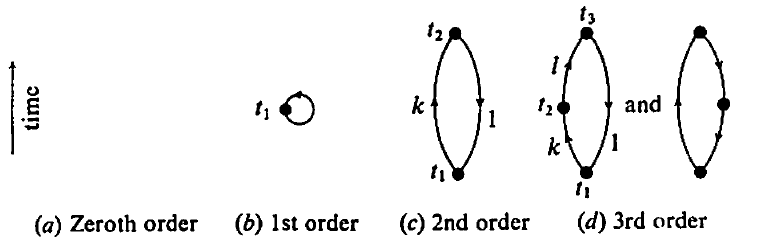
\includegraphics[width=0.8\textwidth]{screenshots/single-electron-diagram-order.PNG}
    \label{single-electron-diagram-order}
\end{equation}
In second order, at $t_1$, $V(\mathbf{t})$ can scatter the particle up into the state $\phi_k$, thus simultaneously creating a hole in $\phi_1$ and a particle in $\phi_k$, and at $t_2$ scatter the particle back into $\phi_1$. The fourth-order ones are
\begin{equation}
    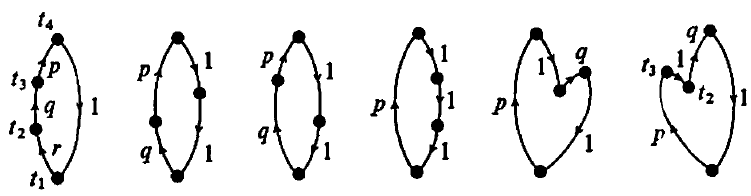
\includegraphics[width=0.8\textwidth]{screenshots/single-electron-4th-order.PNG}
    \label{single-electron-4th-order}
\end{equation}
Note that in the last two diagrams of (\ref{single-electron-4th-order}) there are two particle lines and two hole lines between $t_{2}$ and $t_{3},$ whereas our one-particle system can have at most one particle and one hole. However, it is easily shown that \textbf{these diagrams are exactly cancelled by unlinked diagrams of the sort in (\ref{single-electron-unlinked-diagram}) below}. 
\begin{equation}
    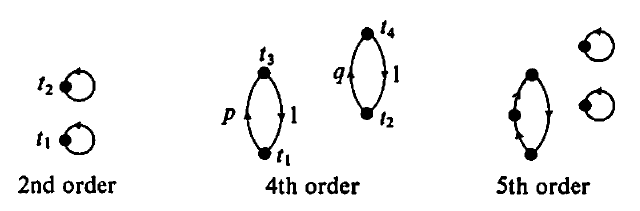
\includegraphics[width=0.8\textwidth]{screenshots/single-electron-unlinked-diagram.PNG}
    \label{single-electron-unlinked-diagram}
\end{equation}
For example, because of \textbf{the (-1) from the extra fermion loop}, the last diagram in (\ref{single-electron-4th-order}) is cancelled by the fourth-order diagram in (\ref{single-electron-unlinked-diagram}). \bluep{Nevertheless, it is necessary to retain such diagrams which violate conservation of particle number, in order to prove the linked cluster theorem.} The same argument holds for diagrams which violate the Pauli exclusion principle.

In order to draw all diagrams in $n$ th order, draw $n$ dots in a vertical row, label them $t_{1}, t_{2}, \ldots, t_{n}$ and connect them up in all possible \textbf{'topologically distinct'} (see below) ways with one line entering and one leaving each dot. For example in third order we find the six diagrams
\begin{center}
    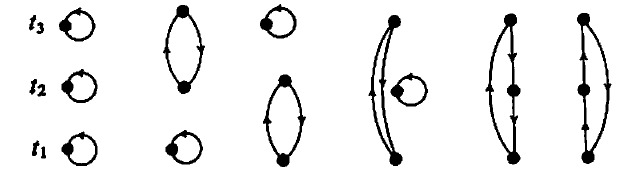
\includegraphics[width=0.8\textwidth]{screenshots/single-electron-topo-distinct.PNG}
\end{center}
Two diagrams are ' \textbf{topologically equivalent}' if one can be \bluep{distorted into the other without changing the vertical ordering of the dots; otherwise they are distinct.} This is illustrated by the fourth-order diagrams (\textbf{note significance of the direction of the arrows}).

Finally, the diagrammatic expansion for the vacuum amplitude will just be the sum of all diagrams such as the above:
\begin{equation}
    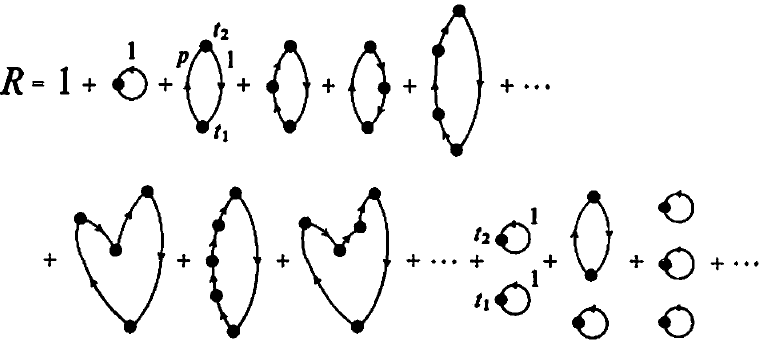
\includegraphics[width=0.8\textwidth]{screenshots/single-electron-ground-expansion.PNG}
    \label{single-electron-ground-expansion}
\end{equation}
where the 1 expresses the fact that in the unperturbed case, the probability amplitude for the system staying in its ground state is 1. Translate the series into equation we have
\begin{equation}
    \begin{aligned}
    R(t)=1-&V_{11} \int_{0}^{t} d t_{1} G_{0}\left(1, t_{1}-t_{1}\right)-\\
    &-\sum_{p>1} V_{1p} V_{p 1} \int_{0}^{t} d t_{1} \int_{0}^{t} \underset{t_2>t_1}{dt_2} G_{0}^{+}\left(p, t_{2}-t_{1}\right) G_{0}^{-}\left(1, t_{1}-t_{2}\right)+\cdots\\
    &+V_{11} V_{11} \int_{0}^{t} d t_{1} \int_{0}^{t} \underset{t_2>t_1}{d t_{2}} \quad G_{0}^{-}\left(1, t_{1}-t_{1}\right) \sigma_{0}\left(1, t_{2}-t_{2}\right)+\cdots
    \end{aligned}
\end{equation}

\subsection{Linked cluster theorem for one-particle system}
The theorem states that
\begin{equation}
    lnR(t)=\Sigma\text{ all linked graphs}
    \label{single-electron-linked-theorem}
\end{equation}
The proof is based on the fact that \textbf{the contribution from a unlinked diagram is proportional to the product of the contribution of its various parts.} Consider for example the $V_{11}V_{11}$ term:
\begin{center}
\tikzset{every picture/.style={line width=0.75pt}} %set default line width to 0.75pt        
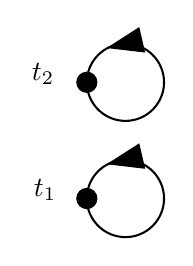
\begin{tikzpicture}[x=0.75pt,y=0.75pt,yscale=-1,xscale=1]
%uncomment if require: \path (0,244); %set diagram left start at 0, and has height of 244

%Shape: Circle [id:dp6498223397318404] 
\draw   (81,85.6) .. controls (81,75.33) and (89.33,67) .. (99.6,67) .. controls (109.87,67) and (118.2,75.33) .. (118.2,85.6) .. controls (118.2,95.87) and (109.87,104.2) .. (99.6,104.2) .. controls (89.33,104.2) and (81,95.87) .. (81,85.6) -- cycle ;
%Shape: Circle [id:dp27995222268876896] 
\draw  [fill={rgb, 255:red, 0; green, 0; blue, 0 }  ,fill opacity=1 ] (76.4,85.6) .. controls (76.4,83.06) and (78.46,81) .. (81,81) .. controls (83.54,81) and (85.6,83.06) .. (85.6,85.6) .. controls (85.6,88.14) and (83.54,90.2) .. (81,90.2) .. controls (78.46,90.2) and (76.4,88.14) .. (76.4,85.6) -- cycle ;
%Shape: Triangle [id:dp3898756772562222] 
\draw  [fill={rgb, 255:red, 0; green, 0; blue, 0 }  ,fill opacity=1 ] (92,68.75) -- (105.94,59.79) -- (108.46,70.7) -- cycle ;
%Shape: Circle [id:dp6531439047197907] 
\draw   (81,141.6) .. controls (81,131.33) and (89.33,123) .. (99.6,123) .. controls (109.87,123) and (118.2,131.33) .. (118.2,141.6) .. controls (118.2,151.87) and (109.87,160.2) .. (99.6,160.2) .. controls (89.33,160.2) and (81,151.87) .. (81,141.6) -- cycle ;
%Shape: Circle [id:dp7775379383850192] 
\draw  [fill={rgb, 255:red, 0; green, 0; blue, 0 }  ,fill opacity=1 ] (76.4,141.6) .. controls (76.4,139.06) and (78.46,137) .. (81,137) .. controls (83.54,137) and (85.6,139.06) .. (85.6,141.6) .. controls (85.6,144.14) and (83.54,146.2) .. (81,146.2) .. controls (78.46,146.2) and (76.4,144.14) .. (76.4,141.6) -- cycle ;
%Shape: Triangle [id:dp43271531457083345] 
\draw  [fill={rgb, 255:red, 0; green, 0; blue, 0 }  ,fill opacity=1 ] (92,124.75) -- (105.94,115.79) -- (108.46,126.7) -- cycle ;

% Text Node
\draw (54,131) node [anchor=north west][inner sep=0.75pt]    {$t_{1}$};
% Text Node
\draw (53,75) node [anchor=north west][inner sep=0.75pt]    {$t_{2}$};
\end{tikzpicture}
\end{center}
Translating it into equation we have
$$
\begin{aligned}
&V_{11} V_{11} \int_{0}^{t} d t_{1} \int_{0}^{t} \underset{t_2>t_1}{d t_{2}} G_{0}^{-} G_{0}^{-}=V_{11}^{2} G_{0}^{-2} \int_{0}^{t} d t_{1} \int_{0}^{t} \underset{t_2>t_1}{d t_{2}}\\
&=V_{11}^{2} G_{0}^{-2} \int_{0}^{t} d t_{1} \int_{0}^{t} d t_{2} \times \frac{1}{2} \quad \text { (where } t_{2}>\text { or }<t_{1})\\
&=\frac{1}{2}\left[V_{11} \int_{0}^{1} d t_{1} G_{0}^{-}\left(1, t_{1}-t_{1}\right)\right] \times\left[V_{11} \int_{0}^{t} d t_{2} G_{0}^{-}\left(1, t_{2}-t_{2}\right)\right]\\
&=\frac{1}{2!}\times\selfcirc^2
\end{aligned}
$$
In general, it turns out that the value of an unlinked diagram with $n$ identical links $L,$ is just $(1 / n !) \times L^{n}$.

A similar factorization occurs for non-identical links if we first sum over all possible time orders. For example, the following three graphs can be summed over:
\begin{center}
\tikzset{every picture/.style={line width=0.75pt}} %set default line width to 0.75pt        
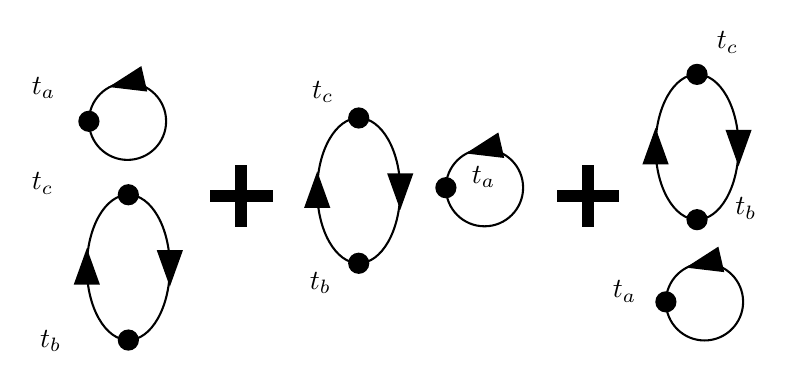
\begin{tikzpicture}[x=0.75pt,y=0.75pt,yscale=-1,xscale=1]
%uncomment if require: \path (0,244); %set diagram left start at 0, and has height of 244

%Shape: Circle [id:dp6498223397318404] 
\draw   (81,85.6) .. controls (81,75.33) and (89.33,67) .. (99.6,67) .. controls (109.87,67) and (118.2,75.33) .. (118.2,85.6) .. controls (118.2,95.87) and (109.87,104.2) .. (99.6,104.2) .. controls (89.33,104.2) and (81,95.87) .. (81,85.6) -- cycle ;
%Shape: Circle [id:dp27995222268876896] 
\draw  [fill={rgb, 255:red, 0; green, 0; blue, 0 }  ,fill opacity=1 ] (76.4,85.6) .. controls (76.4,83.06) and (78.46,81) .. (81,81) .. controls (83.54,81) and (85.6,83.06) .. (85.6,85.6) .. controls (85.6,88.14) and (83.54,90.2) .. (81,90.2) .. controls (78.46,90.2) and (76.4,88.14) .. (76.4,85.6) -- cycle ;
%Shape: Triangle [id:dp3898756772562222] 
\draw  [fill={rgb, 255:red, 0; green, 0; blue, 0 }  ,fill opacity=1 ] (92,68.75) -- (105.94,59.79) -- (108.46,70.7) -- cycle ;
%Shape: Ellipse [id:dp25610156841716825] 
\draw   (100,121) .. controls (111.05,121) and (120,136.67) .. (120,156) .. controls (120,175.33) and (111.05,191) .. (100,191) .. controls (88.95,191) and (80,175.33) .. (80,156) .. controls (80,136.67) and (88.95,121) .. (100,121) -- cycle ;
%Shape: Circle [id:dp9579907217839725] 
\draw  [fill={rgb, 255:red, 0; green, 0; blue, 0 }  ,fill opacity=1 ] (95.4,121) .. controls (95.4,118.46) and (97.46,116.4) .. (100,116.4) .. controls (102.54,116.4) and (104.6,118.46) .. (104.6,121) .. controls (104.6,123.54) and (102.54,125.6) .. (100,125.6) .. controls (97.46,125.6) and (95.4,123.54) .. (95.4,121) -- cycle ;
%Shape: Circle [id:dp44384941541376566] 
\draw  [fill={rgb, 255:red, 0; green, 0; blue, 0 }  ,fill opacity=1 ] (95.4,191) .. controls (95.4,188.46) and (97.46,186.4) .. (100,186.4) .. controls (102.54,186.4) and (104.6,188.46) .. (104.6,191) .. controls (104.6,193.54) and (102.54,195.6) .. (100,195.6) .. controls (97.46,195.6) and (95.4,193.54) .. (95.4,191) -- cycle ;
%Shape: Triangle [id:dp08449835110518966] 
\draw  [fill={rgb, 255:red, 0; green, 0; blue, 0 }  ,fill opacity=1 ] (120,163.8) -- (114.4,148.2) -- (125.6,148.2) -- cycle ;
%Shape: Triangle [id:dp33847857915014856] 
\draw  [fill={rgb, 255:red, 0; green, 0; blue, 0 }  ,fill opacity=1 ] (80,148.2) -- (85.6,163.8) -- (74.4,163.8) -- cycle ;
%Shape: Circle [id:dp16953709843220488] 
\draw   (253,117.6) .. controls (253,107.33) and (261.33,99) .. (271.6,99) .. controls (281.87,99) and (290.2,107.33) .. (290.2,117.6) .. controls (290.2,127.87) and (281.87,136.2) .. (271.6,136.2) .. controls (261.33,136.2) and (253,127.87) .. (253,117.6) -- cycle ;
%Shape: Circle [id:dp23125089891886985] 
\draw  [fill={rgb, 255:red, 0; green, 0; blue, 0 }  ,fill opacity=1 ] (248.4,117.6) .. controls (248.4,115.06) and (250.46,113) .. (253,113) .. controls (255.54,113) and (257.6,115.06) .. (257.6,117.6) .. controls (257.6,120.14) and (255.54,122.2) .. (253,122.2) .. controls (250.46,122.2) and (248.4,120.14) .. (248.4,117.6) -- cycle ;
%Shape: Triangle [id:dp3247983028310686] 
\draw  [fill={rgb, 255:red, 0; green, 0; blue, 0 }  ,fill opacity=1 ] (264,100.75) -- (277.94,91.79) -- (280.46,102.7) -- cycle ;
%Shape: Ellipse [id:dp473301006793975] 
\draw   (211,84) .. controls (222.05,84) and (231,99.67) .. (231,119) .. controls (231,138.33) and (222.05,154) .. (211,154) .. controls (199.95,154) and (191,138.33) .. (191,119) .. controls (191,99.67) and (199.95,84) .. (211,84) -- cycle ;
%Shape: Circle [id:dp7910773789667759] 
\draw  [fill={rgb, 255:red, 0; green, 0; blue, 0 }  ,fill opacity=1 ] (206.4,84) .. controls (206.4,81.46) and (208.46,79.4) .. (211,79.4) .. controls (213.54,79.4) and (215.6,81.46) .. (215.6,84) .. controls (215.6,86.54) and (213.54,88.6) .. (211,88.6) .. controls (208.46,88.6) and (206.4,86.54) .. (206.4,84) -- cycle ;
%Shape: Circle [id:dp29762035839742207] 
\draw  [fill={rgb, 255:red, 0; green, 0; blue, 0 }  ,fill opacity=1 ] (206.4,154) .. controls (206.4,151.46) and (208.46,149.4) .. (211,149.4) .. controls (213.54,149.4) and (215.6,151.46) .. (215.6,154) .. controls (215.6,156.54) and (213.54,158.6) .. (211,158.6) .. controls (208.46,158.6) and (206.4,156.54) .. (206.4,154) -- cycle ;
%Shape: Triangle [id:dp5382643640790852] 
\draw  [fill={rgb, 255:red, 0; green, 0; blue, 0 }  ,fill opacity=1 ] (231,126.8) -- (225.4,111.2) -- (236.6,111.2) -- cycle ;
%Shape: Triangle [id:dp787103954892548] 
\draw  [fill={rgb, 255:red, 0; green, 0; blue, 0 }  ,fill opacity=1 ] (191,111.2) -- (196.6,126.8) -- (185.4,126.8) -- cycle ;
%Shape: Circle [id:dp4980802915672331] 
\draw   (359,172.6) .. controls (359,162.33) and (367.33,154) .. (377.6,154) .. controls (387.87,154) and (396.2,162.33) .. (396.2,172.6) .. controls (396.2,182.87) and (387.87,191.2) .. (377.6,191.2) .. controls (367.33,191.2) and (359,182.87) .. (359,172.6) -- cycle ;
%Shape: Circle [id:dp9401870635500967] 
\draw  [fill={rgb, 255:red, 0; green, 0; blue, 0 }  ,fill opacity=1 ] (354.4,172.6) .. controls (354.4,170.06) and (356.46,168) .. (359,168) .. controls (361.54,168) and (363.6,170.06) .. (363.6,172.6) .. controls (363.6,175.14) and (361.54,177.2) .. (359,177.2) .. controls (356.46,177.2) and (354.4,175.14) .. (354.4,172.6) -- cycle ;
%Shape: Triangle [id:dp7535245748392855] 
\draw  [fill={rgb, 255:red, 0; green, 0; blue, 0 }  ,fill opacity=1 ] (370,155.75) -- (383.94,146.79) -- (386.46,157.7) -- cycle ;
%Shape: Ellipse [id:dp796880375497128] 
\draw   (374,63) .. controls (385.05,63) and (394,78.67) .. (394,98) .. controls (394,117.33) and (385.05,133) .. (374,133) .. controls (362.95,133) and (354,117.33) .. (354,98) .. controls (354,78.67) and (362.95,63) .. (374,63) -- cycle ;
%Shape: Circle [id:dp2607772888080764] 
\draw  [fill={rgb, 255:red, 0; green, 0; blue, 0 }  ,fill opacity=1 ] (369.4,63) .. controls (369.4,60.46) and (371.46,58.4) .. (374,58.4) .. controls (376.54,58.4) and (378.6,60.46) .. (378.6,63) .. controls (378.6,65.54) and (376.54,67.6) .. (374,67.6) .. controls (371.46,67.6) and (369.4,65.54) .. (369.4,63) -- cycle ;
%Shape: Circle [id:dp36338449977521137] 
\draw  [fill={rgb, 255:red, 0; green, 0; blue, 0 }  ,fill opacity=1 ] (369.4,133) .. controls (369.4,130.46) and (371.46,128.4) .. (374,128.4) .. controls (376.54,128.4) and (378.6,130.46) .. (378.6,133) .. controls (378.6,135.54) and (376.54,137.6) .. (374,137.6) .. controls (371.46,137.6) and (369.4,135.54) .. (369.4,133) -- cycle ;
%Shape: Triangle [id:dp6814504901438665] 
\draw  [fill={rgb, 255:red, 0; green, 0; blue, 0 }  ,fill opacity=1 ] (394,105.8) -- (388.4,90.2) -- (399.6,90.2) -- cycle ;
%Shape: Triangle [id:dp44737264879533356] 
\draw  [fill={rgb, 255:red, 0; green, 0; blue, 0 }  ,fill opacity=1 ] (354,90.2) -- (359.6,105.8) -- (348.4,105.8) -- cycle ;
%Shape: Cross [id:dp06220635309920053] 
\draw  [fill={rgb, 255:red, 0; green, 0; blue, 0 }  ,fill opacity=1 ] (152.1,107) -- (156.9,107) -- (156.9,119.1) -- (169,119.1) -- (169,123.9) -- (156.9,123.9) -- (156.9,136) -- (152.1,136) -- (152.1,123.9) -- (140,123.9) -- (140,119.1) -- (152.1,119.1) -- cycle ;
%Shape: Cross [id:dp6139216079282784] 
\draw  [fill={rgb, 255:red, 0; green, 0; blue, 0 }  ,fill opacity=1 ] (319.1,107) -- (323.9,107) -- (323.9,119.1) -- (336,119.1) -- (336,123.9) -- (323.9,123.9) -- (323.9,136) -- (319.1,136) -- (319.1,123.9) -- (307,123.9) -- (307,119.1) -- (319.1,119.1) -- cycle ;

% Text Node
\draw (52,109) node [anchor=north west][inner sep=0.75pt]    {$t_{c}$};
% Text Node
\draw (56,185) node [anchor=north west][inner sep=0.75pt]    {$t_{b}$};
% Text Node
\draw (52,63) node [anchor=north west][inner sep=0.75pt]    {$t_{a}$};
% Text Node
\draw (264,106) node [anchor=north west][inner sep=0.75pt]    {$t_{a}$};
% Text Node
\draw (187,65) node [anchor=north west][inner sep=0.75pt]    {$t_{c}$};
% Text Node
\draw (186,157) node [anchor=north west][inner sep=0.75pt]    {$t_{b}$};
% Text Node
\draw (391,121) node [anchor=north west][inner sep=0.75pt]    {$t_{b}$};
% Text Node
\draw (382,41) node [anchor=north west][inner sep=0.75pt]    {$t_{c}$};
% Text Node
\draw (332,161) node [anchor=north west][inner sep=0.75pt]    {$t_{a}$};


\end{tikzpicture}
\end{center}
Translate into equations we have
\begin{equation}\begin{array}{l}
\sum_{k} V_{k 1} V_{1 k} V_{11} \iiint d t_{a} d t_{b} d t_{c} \times \\
\quad \times G_{0}^{+}\left(k, t_{c}-t_{b}\right) G_{0}^{-}\left(1, t_{b}-t_{c}\right) G_{0}^{-}\left(1, t_{a}-t_{a}\right) \times \\
\quad \times\left[\theta_{t_a-t_c}, \theta_{t_c-t_{b}}+\theta_{t_c-t_{a}} \theta_{t_{a}-t_{b}}+\theta_{t_c-t_b} \theta_{t_{b}-t_c}\right]\\
=\selfcirc\times\fermiloop
\end{array}\end{equation}
The $\theta^{\prime} s$ are used as a convenient way of writing the time order in the three diagrams. For $t_{c}>t_{b},$ some concentration shows that the term in brackets $=1$ regardless of where $t_{a}$ lies. This means the integral over $t_{a}$ is independent of that over $t_{b}$ and $t_{c},$ so the triple integral factorizes into two parts producing the result shown.

Combining these results, one finds that R may be written
\begin{equation}
\begin{aligned}
&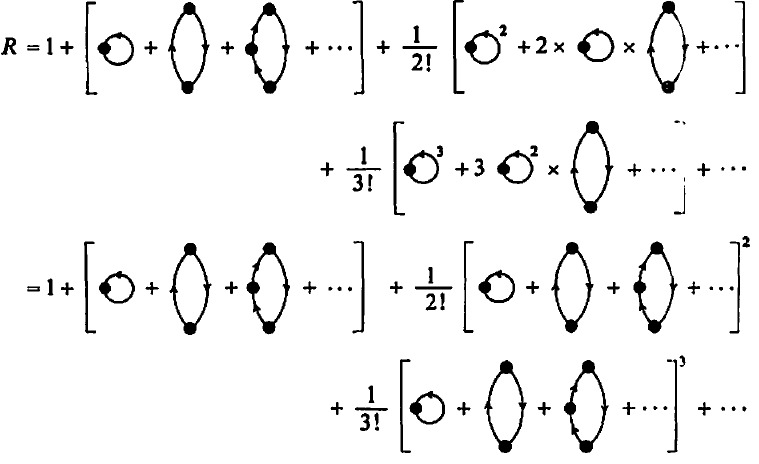
\includegraphics[width=0.8\textwidth]{screenshots/single-electron-R.PNG}\\
&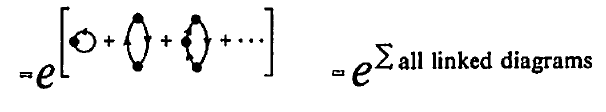
\includegraphics[width=0.8\textwidth]{screenshots/single-electron-R2.PNG}
\end{aligned}
\label{single-electron-R}
\end{equation}
In the many-body case, there is a deeper reason for the importance of the linked cluster theorem, e.g., \bluep{if we do not use it, we find that the perturbation series for the energy appears to diverge badly as the number of particles $N\rightarrow\infty$}.
\subsection{Finding the ground state energy in one-particle system}
Because the ground state energy depends only on the logarithm of $R$:
$$
E_{0}=\epsilon_{1}+\lim _{t \rightarrow \infty(1-i \eta)} i \frac{d}{d t} \ln R(t)
$$
it is now possible to obtain the expression for the ground state energy by translating the above diagrams into the following equations(remember \bluep{the (-1) factor in front of the "limit" is for the "fermion loop"}):
\begin{equation}
    \begin{aligned}
    E_{0}=&\epsilon_{1}-\lim _{n \rightarrow \infty(1-i\eta )} i \frac{d}{d t}\left\{(-i) V_{11} \int_{0}^{t} d t_{1} i G_{0}^{-}\left(1, t_{1}-t_{1}\right)+\right.\\
    &\left.+\sum_{p \neq 1}(-i)^{2} V_{1 p} V_{p 1} \int_{0}^{t} d t_{1} \int_{0}^{t} \underset{t_2>t_1}{d t_{2}} i G_{0}^{+}\left(p, t_{2}-t_{1}\right) i G_{0}^{-}\left(1, t_{1}-t_{2}\right)+\cdots\right\}
    \end{aligned}
\end{equation}
Thus, 
$$
E_0^{(1)}=\lim_{t\rightarrow\infty(1-i\eta)}i\frac{d}{dt}\selfcirc=V_{11}
$$
and the second term produces
$$
\begin{aligned}
\fermiloop&=(-1)^{2}(-i)^{2} \sum_{p \neq 1} V_{1 p} V_{p 1} \int_{0}^{1} d t_{1} \int_{0}^{t} d t_{2} \theta_{t_2-t_1} e^{-i\left(\epsilon_{p}-\epsilon_{1}\right)\left(t_{2}-t_{1}\right)}\\
&=(-1)^{2}(-i)^{2} \sum_{p \neq 1} V_{1 p} V_{p 1} \int_{0}^{t} d t_{1} \int_{0}^{t-t_{1}} d\left(t_{2}-t_{1}\right) e^{-i\left(\epsilon_{p}-\epsilon_1\right)\left(t_{2}-t_{1}\right)}
\end{aligned}
$$
Thus
$$
\lim _{t \rightarrow \infty(1-i\eta)} i \frac{d}{d t}\fermiloop=-i \sum_{p \neq 1} V_{1 p} V_{p 1}\left[-\frac{e^{-i\left(\epsilon_{p}-\epsilon_{1}\right) \omega(1-i \eta)}}{i\left(\epsilon_{p}-\epsilon_{1}\right)}+\frac{1}{i\left(\epsilon_{p}-\epsilon_{1}\right)}\right]
$$
or
\begin{equation}E_{0}^{(2)}=\sum_{p \neq 1} \frac{V_{1 p} V_{p 1}}{\epsilon_{1}-\epsilon_{p}}\end{equation}
where \redp{\textbf{the oscillating exponential is killed because $\left(\epsilon_{1}-\epsilon_{p}\right)$ and the infinitesimal $\eta \text { are both positive. (Note that } \eta \text { is chosen such that } \eta \times \infty=\infty .)$}} Proceeding in this way yields the third-and fourth-order terms:
\begin{equation}E_{0}^{(3)}=\sum_{p, q \neq 1} \frac{V_{1 p} V_{p q} V_{q 1}}{\left(\epsilon_{1}-\epsilon_{p}\right)\left(\epsilon_{1}-\epsilon_{q}\right)}-\sum_{p \neq 1} \frac{V_{1p}V_{p1} V_{11}}{\left(\epsilon_{1}-\epsilon_{p}\right)^{2}}
\label{single-electron-third-order}
\end{equation}
\begin{equation}
\begin{aligned}
E_{0}^{(4)}=& \sum_{p, q, r \neq 1} \frac{V_{1 p} V_{p q} V_{q r} V_{r 1}}{\left(\epsilon_{1}-\epsilon_{p}\right)\left(\epsilon_{1}-\epsilon_{q}\right)\left(\epsilon_{1}-\epsilon_{r}\right)}-\sum_{p, q \neq1} \frac{V_{1p} V_{p q} V_{q 1} V_{11}}{\left(\epsilon_{1}-\epsilon_{p}\right)^{2}\left(\epsilon_{1}-\epsilon_{q}\right)}-\\
&-\sum_{p, q \neq 1} \frac{V_{1 p} V_{p q} V_{q 1} V_{11}}{\left(\epsilon_{1}-\epsilon_{p}\right)\left(\epsilon_{1}-\epsilon_{q}\right)^{2}}+\sum_{p \neq 1} \frac{V_{1p} V_{p 1} V_{11} V_{11}}{\left(\epsilon_{1}-\epsilon_{p}\right)^{3}}-\\
&-\sum_{p, q \neq 1} \frac{V_{1 p} V_{p 1} V_{1 q} V_{q 1}}{\left(\epsilon_{1}-\epsilon_{p}\right)^{2}\left(\epsilon_{1}-\epsilon_{q}\right)}
\end{aligned}
\label{single-electron-fourth-order}
\end{equation}
This is the well-known Rayleigh-Schrodinger perturbation series carried out to fourth order. Now we use diagrammatic method to carry out the calculation to infinite order by \textbf{providing a systematic method for writing out the $nth-$order term in the expansion of $E_0$.}
\begin{imp}
To get the numerator of each term in (\ref{single-electron-third-order}-\ref{single-electron-fourth-order}), the product of $V_{kl}$ factors associated with the interaction dots will do. To get the denominator, draw light dotted horizontal lines \redp{between successive (in time) pairs of vertices}, thus
\begin{center}
    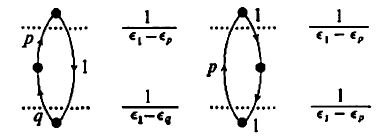
\includegraphics[width=0.8\textwidth]{screenshots/single-electron-denominator-rule.PNG}
\end{center}
and associated a factor of
\begin{equation}
    \frac{1}{\underset{\parbox{100pt}{\centering\tiny{all hole lines intersected by dotted line}}}{\Sigma \epsilon_1}-\underset{\parbox{100pt}{\centering\tiny{all particle lines intersected by dotted line}}}{\Sigma\epsilon_p}}
\end{equation}
The proper sign is obtained by multiplying by the factor $(-1)^{h+1}$ where h=number of hole lines in the diagram. The final rule is to sum over all particle indices.
\end{imp}
Applying these rules (which can be rigorously proved from the vacuum amplitude expansion) yields both of the third-order terms and they also produce the correct result in the other orders. (Note that in fourth order, the last term in (\ref{single-electron-fourth-order}) is obtained by summing the two "mitten" diagrams of (\ref{single-electron-4th-order}).)

Imagine that the perturbing potential is so large that it is impossible to get a decent result by using the usual method of cutting off the series after the first few orders. But suppose, for example, that the potential happens to have big matrix elements only between the ground and first excited states, i.e.,that $V_{12}$ and $V_{21}$ are large but all others are small. Then the perturbation series may be approximated by a partial sum over just those special diagrams in which all vertices connect '1' lines and '2' lines. This means that $E_0$ reduces to a sum over just the following diagrams
\begin{equation}
    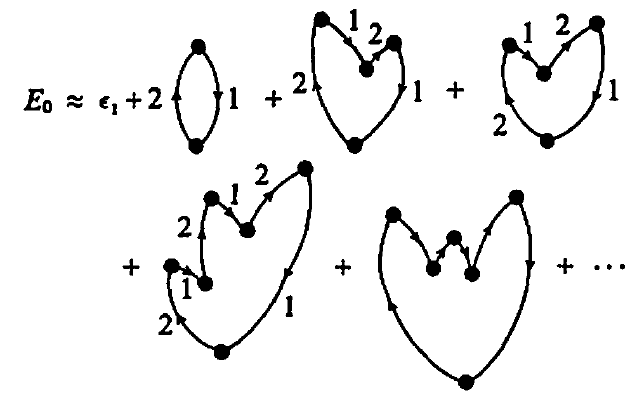
\includegraphics[width=0.8\textwidth]{screenshots/single-electron-V12-series.PNG}
    \label{single-electron-V12-series}
\end{equation}
\bluep{Note that the odd-order diagrams do not occur. And each term representing a graph type is multiplied with a degeneracy factor}. Using the rules this series yields
\begin{equation}\begin{aligned}
E_{0} \approx \epsilon_{1} &+\frac{\left|V_{12}\right|^{2}}{\epsilon_{1}-\epsilon_{2}}-\frac{\left|V_{12}\right|^{4}}{\left(\epsilon_{1}-\epsilon_{2}\right) \times 2\left(\epsilon_{1}-\epsilon_{2}\right) \times\left(\epsilon_{1}-\epsilon_{2}\right)} \times 2 \\
&+\frac{\left|V_{12}\right|^{6}}{\left(\epsilon_{1}-\epsilon_{2}\right) \times 2\left(\epsilon_{1}-\epsilon_{2}\right) \times\left(\epsilon_{1}-\epsilon_{2}\right) \times 2\left(\epsilon_{1}-\epsilon_{2}\right) \times\left(\epsilon_{1}-\epsilon_{2}\right)} \times 4 \\
&+\frac{\left|V_{12}\right|^{6}}{\left(\epsilon_{1}-\epsilon_{2}\right) \times 2\left(\epsilon_{1}-\epsilon_{2}\right) \times 3\left(\epsilon_{1}-\epsilon_{2}\right) \times 2\left(\epsilon_{1}-\epsilon_{2}\right) \times\left(\epsilon_{1}-\epsilon_{2}\right)} \times 12 \\
&+\cdots\\
&=\epsilon_{1}+\frac{\left|V_{12}\right|^{2}}{\epsilon_{1}-\epsilon_{2}}-\frac{\left|V_{12}\right|^{4}}{\left(\epsilon_{1}-\epsilon_{2}\right)^{3}}+\frac{2\left|V_{12}\right|^{6}}{\left(\epsilon_{1}-\epsilon_{2}\right)^{5}}+\cdots
\end{aligned}\end{equation}
\redp{Note that the term $2(\epsilon_1-\epsilon_2)$ comes from the fact that the vertical line intersects with 2 hole lines and 2 particle liens}. By adding and subtracting $\epsilon_{1} / 2$ and factoring out $\frac{1}{2}\left(\epsilon_{1}-\epsilon_{2}\right)$ yielding
\begin{equation}E_{0}=\frac{\epsilon_{1}+\epsilon_{2}}{2}+\frac{\left(\epsilon_{1}-\epsilon_{2}\right)}{2}\left[1+\frac{2\left|V_{12}\right|^{2}}{\left(\epsilon_{1}-\epsilon_{2}\right)^{2}}-\frac{2\left|V_{12}\right|^{4}}{\left(\epsilon_{1}-\epsilon_{2}\right)^{4}}+\frac{4\left|V_{12}\right|^{6}}{\left(\epsilon_{1}-\epsilon_{2}\right)^{6}}+\cdots\right]\end{equation}
The bracketed term is seen to be just the infinite series for the square root, giving us the final result
\begin{equation}E_{0} \approx \frac{\epsilon_{1}+\epsilon_{2}}{2}+\frac{\left(\epsilon_{1}-\epsilon_{2}\right)}{2} \sqrt{\left\{1+\frac{4\left|V_{12}\right|^{2}}{\left(\epsilon_{1}-\epsilon_{2}\right)^{2}}\right\}}\end{equation}
\subsection{The many-body case}
The vacuum amplitude may then be built up as the sum of all possible sequences of interactions beginning and ending in the many-body ground state, or vacuum. The ground state energy again involves just the sum over linked diagrams and may be written as follows:
\begin{equation}
    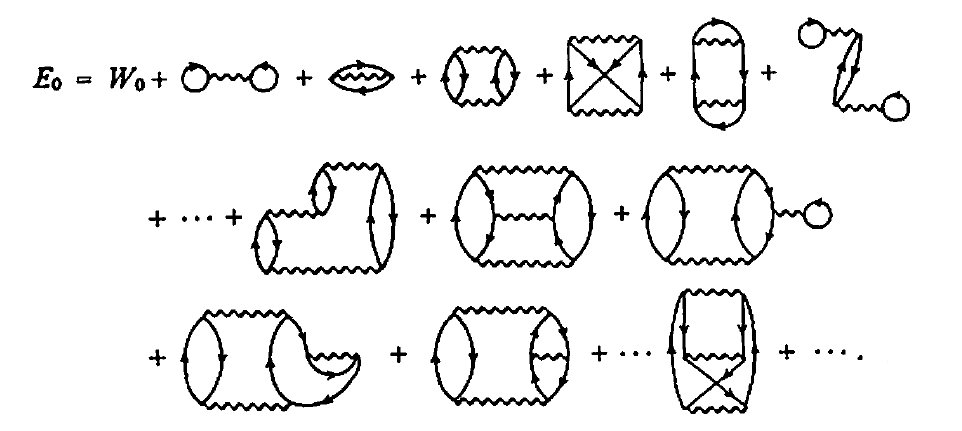
\includegraphics[width=0.8\textwidth]{screenshots/many-body-vacuum-series.PNG}
    \label{many-body-vacuum-series}
\end{equation}
Here we will content ourselves with briefly mentioning a few popular approximations for the ground state energy which can be made with (\ref{many-body-vacuum-series}).

The simplest approximation is the \textbf{\redp{Hartree-Fock (HF), which is just the sum of the double-bubble and oyster diagrams}}:
\begin{equation}
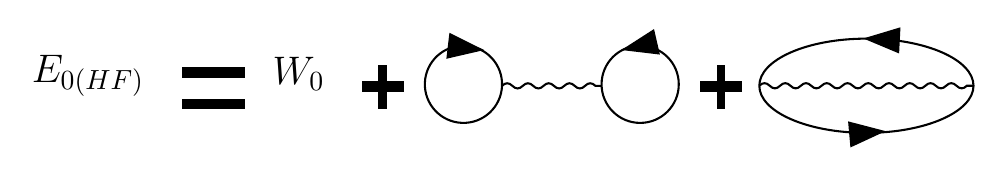
\begin{tikzpicture}[x=0.75pt,y=0.75pt,yscale=-1,xscale=1]
%uncomment if require: \path (0,244); %set diagram left start at 0, and has height of 244

%Shape: Circle [id:dp6498223397318404] 
\draw   (302,124.6) .. controls (302,114.33) and (310.33,106) .. (320.6,106) .. controls (330.87,106) and (339.2,114.33) .. (339.2,124.6) .. controls (339.2,134.87) and (330.87,143.2) .. (320.6,143.2) .. controls (310.33,143.2) and (302,134.87) .. (302,124.6) -- cycle ;
%Shape: Triangle [id:dp3898756772562222] 
\draw  [fill={rgb, 255:red, 0; green, 0; blue, 0 }  ,fill opacity=1 ] (313,107.75) -- (326.94,98.79) -- (329.46,109.7) -- cycle ;
%Shape: Cross [id:dp06220635309920053] 
\draw  [fill={rgb, 255:red, 0; green, 0; blue, 0 }  ,fill opacity=1 ] (195.01,115.6) -- (198.19,115.6) -- (198.19,123.61) -- (206.2,123.61) -- (206.2,127.99) -- (198.19,127.99) -- (198.19,136) -- (195.01,136) -- (195.01,127.99) -- (187,127.99) -- (187,123.61) -- (195.01,123.61) -- cycle ;
%Shape: Circle [id:dp6991360552110061] 
\draw   (216.87,123.85) .. controls (217.28,113.58) and (225.94,105.6) .. (236.2,106.01) .. controls (246.47,106.43) and (254.45,115.08) .. (254.04,125.35) .. controls (253.63,135.61) and (244.97,143.6) .. (234.71,143.18) .. controls (224.44,142.77) and (216.46,134.11) .. (216.87,123.85) -- cycle ;
%Shape: Triangle [id:dp7130261056413152] 
\draw  [fill={rgb, 255:red, 0; green, 0; blue, 0 }  ,fill opacity=1 ] (243.95,107.93) -- (227.8,111.66) -- (229.11,100.54) -- cycle ;
%Straight Lines [id:da10547511660578635] 
\draw    (254.04,125.35) .. controls (255.71,123.68) and (257.37,123.68) .. (259.04,125.35) .. controls (260.71,127.02) and (262.37,127.02) .. (264.04,125.35) .. controls (265.71,123.68) and (267.37,123.68) .. (269.04,125.35) .. controls (270.71,127.02) and (272.37,127.02) .. (274.04,125.35) .. controls (275.71,123.68) and (277.37,123.68) .. (279.04,125.35) .. controls (280.71,127.02) and (282.37,127.02) .. (284.04,125.35) .. controls (285.71,123.68) and (287.37,123.68) .. (289.04,125.35) .. controls (290.71,127.02) and (292.37,127.02) .. (294.04,125.35) .. controls (295.71,123.68) and (297.37,123.68) .. (299.04,125.35) -- (302,125.35) -- (302,125.35) ;
%Shape: Ellipse [id:dp18198799795452325] 
\draw   (378,125.3) .. controls (378,112.76) and (401.1,102.6) .. (429.6,102.6) .. controls (458.1,102.6) and (481.2,112.76) .. (481.2,125.3) .. controls (481.2,137.84) and (458.1,148) .. (429.6,148) .. controls (401.1,148) and (378,137.84) .. (378,125.3) -- cycle ;
%Shape: Triangle [id:dp6530702261537764] 
\draw  [fill={rgb, 255:red, 0; green, 0; blue, 0 }  ,fill opacity=1 ] (429.6,102.6) -- (445.47,97.82) -- (444.89,109.01) -- cycle ;
%Shape: Triangle [id:dp7883771420902802] 
\draw  [fill={rgb, 255:red, 0; green, 0; blue, 0 }  ,fill opacity=1 ] (437.37,147.3) -- (422.33,154.28) -- (421.33,143.12) -- cycle ;
%Straight Lines [id:da8945451528371555] 
\draw    (378,125.3) .. controls (379.67,123.63) and (381.33,123.63) .. (383,125.3) .. controls (384.67,126.97) and (386.33,126.97) .. (388,125.3) .. controls (389.67,123.63) and (391.33,123.63) .. (393,125.3) .. controls (394.67,126.97) and (396.33,126.97) .. (398,125.3) .. controls (399.67,123.63) and (401.33,123.63) .. (403,125.3) .. controls (404.67,126.97) and (406.33,126.97) .. (408,125.3) .. controls (409.67,123.63) and (411.33,123.63) .. (413,125.3) .. controls (414.67,126.97) and (416.33,126.97) .. (418,125.3) .. controls (419.67,123.63) and (421.33,123.63) .. (423,125.3) .. controls (424.67,126.97) and (426.33,126.97) .. (428,125.3) .. controls (429.67,123.63) and (431.33,123.63) .. (433,125.3) .. controls (434.67,126.97) and (436.33,126.97) .. (438,125.3) .. controls (439.67,123.63) and (441.33,123.63) .. (443,125.3) .. controls (444.67,126.97) and (446.33,126.97) .. (448,125.3) .. controls (449.67,123.63) and (451.33,123.63) .. (453,125.3) .. controls (454.67,126.97) and (456.33,126.97) .. (458,125.3) .. controls (459.67,123.63) and (461.33,123.63) .. (463,125.3) .. controls (464.67,126.97) and (466.33,126.97) .. (468,125.3) .. controls (469.67,123.63) and (471.33,123.63) .. (473,125.3) .. controls (474.67,126.97) and (476.33,126.97) .. (478,125.3) -- (481.2,125.3) -- (481.2,125.3) ;
%Shape: Cross [id:dp5950770882977249] 
\draw  [fill={rgb, 255:red, 0; green, 0; blue, 0 }  ,fill opacity=1 ] (358.01,115.6) -- (361.19,115.6) -- (361.19,123.61) -- (369.2,123.61) -- (369.2,127.99) -- (361.19,127.99) -- (361.19,136) -- (358.01,136) -- (358.01,127.99) -- (350,127.99) -- (350,123.61) -- (358.01,123.61) -- cycle ;
%Straight Lines [id:da7229955775391892] 
\draw [line width=3.75]    (100,119) -- (130.2,119) ;
%Straight Lines [id:da17096551384597625] 
\draw [line width=3.75]    (100,134) -- (130.2,134) ;

% Text Node
\draw (142,110) node [anchor=north west][inner sep=0.75pt]  [font=\Large]  {$W_{0}$};
% Text Node
\draw (26,109) node [anchor=north west][inner sep=0.75pt]  [font=\Large]  {$E_{0( HF)}$};


\end{tikzpicture}
\end{equation}
These diagrams involve only three simple rules, so we will evaluate them bere. The rules are: (1) $V_{klmn}$ for each interaction,(2) factor (-1) for each hole line and each fermion loop, and (3) a factor of $\frac{1}{2}$ because the graphs are symmetric. Remembering that all lines are hole lines here, we find
$$E_{0(H F)}=\sum_{k<k_{F}} \epsilon_{k}+\frac{1}{2} \sum_{k, l<k_{F}} V_{k l k l}-\frac{1}{2} \sum_{k ,l<k_{F}} V_{l k k l}$$
The approximation which is good for the high density electron gas (random phase approximation, or 'RPA') involves a partial sum over all 'ring' diagrams in second and higher order:
\begin{equation}
    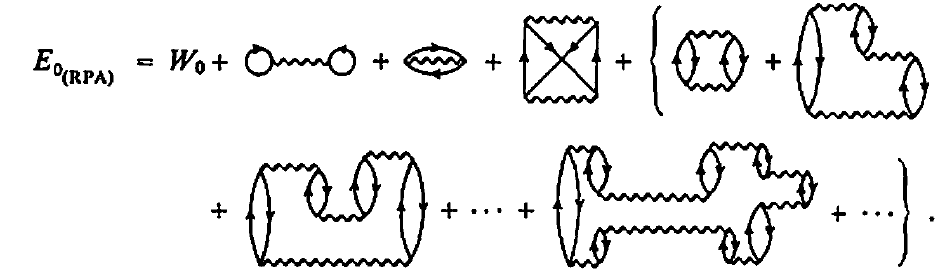
\includegraphics[width=0.8\textwidth]{screenshots/many-body-vacuum-RPA-series.PNG}
\end{equation}
In the case of nuclear matter, we have the 'ladder approximation' involving a partial sum over all ladders:
\begin{equation}
    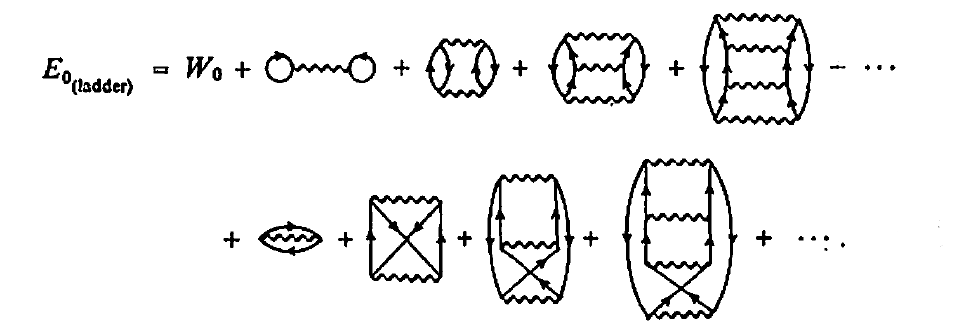
\includegraphics[width=0.8\textwidth]{screenshots/many-body-vacuum-ladder-series.PNG}
\end{equation}